\section{Обзор существующих решений}
\label{sec:Chapter2} \index{Chapter2}
\subsection{Поиск данных в поисковых сервисах}
\subsubsection{Google Dorks (Google Hacking)}
Google Dorks\footnote{https://www.google.com/} -- это по сути та же самая поисковая система от Google. Отличие заключается
только в том, что обычный пользователь вбивает типовые запросы а-ля <<Какая погода в Москве?>>, то Google Dorks позволяет
использовать специальные запросы для получения конкрентной информации. Google Dorks имеет множество операторов, которые 
можно использовать для составления очень гибких и точных запросов \cite{googleHackingWikipedia}. По факту, это запросы, с помощью которых можно проверить
безопасность того или иного сайта, найти IP-адреса сервисов, камер. Весьма эффективна для поиска документации по ключевым словам, 
а также поиску людей с помощью тех же самых Google Dorks Queries. 

\parПлюсы данный системы:
\begin{itemize}
    \item быстрый и объемный поиск по ключевым словам.
\end{itemize}

\parИз недостатков системы можно определить следующее:
\begin{itemize}
    \item составленный запрос выдаст перечень ссылок в интерфейсе поисковой системы, а не сами данные;
    \item перед использованием необоходимо изучить синтаксис запросов;
    \item нет накопления собранной информации, нельзя отслеживать изменения (дельты);
    \item нет построения графа зависимостей объекта.
\end{itemize}

\begin{figure}[H]
    \center{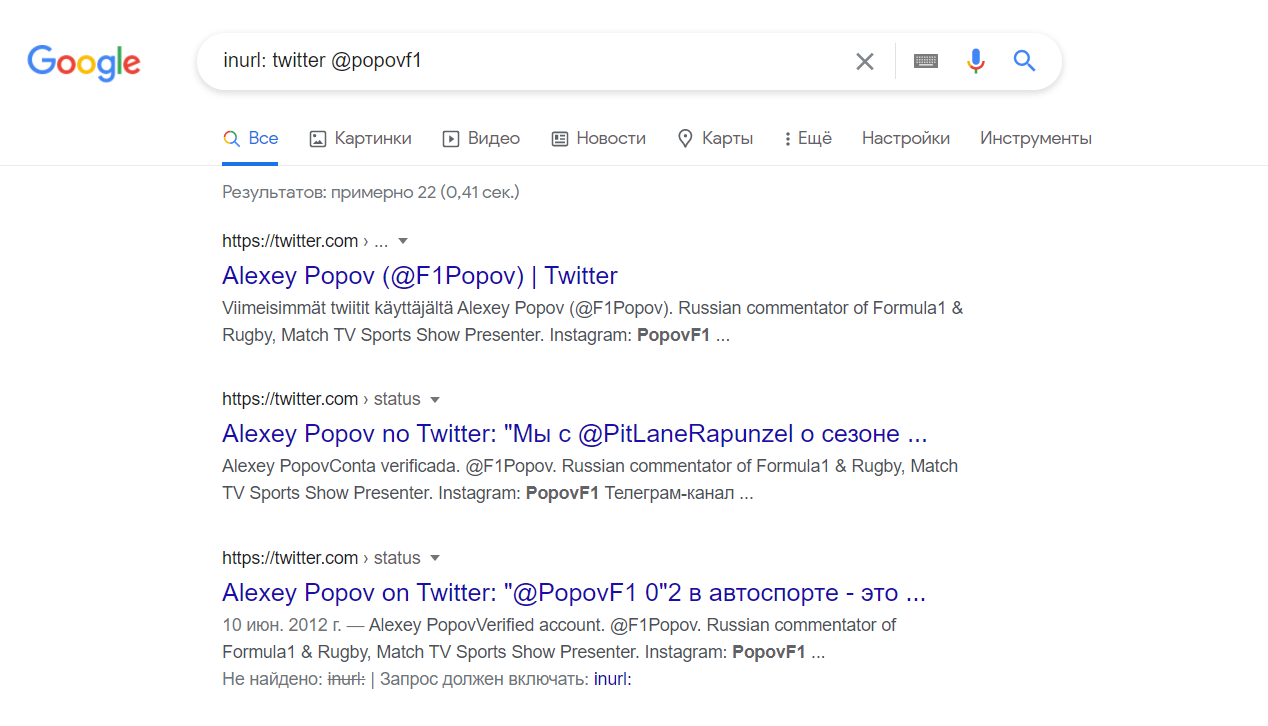
\includegraphics[height=6cm,keepaspectratio]{pictures/GoogleDorksTwitter.png}}
    \caption{Пример использования GDQ для поиска человека.}
    \label{ris:image}
\end{figure}

\subsubsection{Carrot2}
Carrot2 -- движок кластеризации результатов поисковых запросов с открытым исходным кодом. Carrot2 может самостоятельно
группировать по категориям найденные документы или данные. Работает в свою очередь как обычный поисковик, то есть
по указанному ключевому слову возвращает некоторое множество ссылок, затем которые группируются по категориям 
\cite{carrot2wikipedia}.

\par
Преимущества:
\begin{itemize}
    \item быстрый и обширный поиск по ключевым словам;
    \item автоматическая группировка данных в соответствии с категориями;
    \item наличие удобного интерфейса с возможностью просмотра древовидной карты и круговидной диаграммы.
\end{itemize}

\par
Недостатки:
\begin{itemize}
    \item как и в случае с Google Dorks, Carrot2 возвращает нам перечень ссылок на источники данных, а не сами данные
     непосредственно;
    \item невозможно произвести точечный поиск файлов и данных, как это реализовано в Google Dorks. Как следствие -- 
    большое количество лишней информации.
\end{itemize}


\begin{figure}[H]
    \center{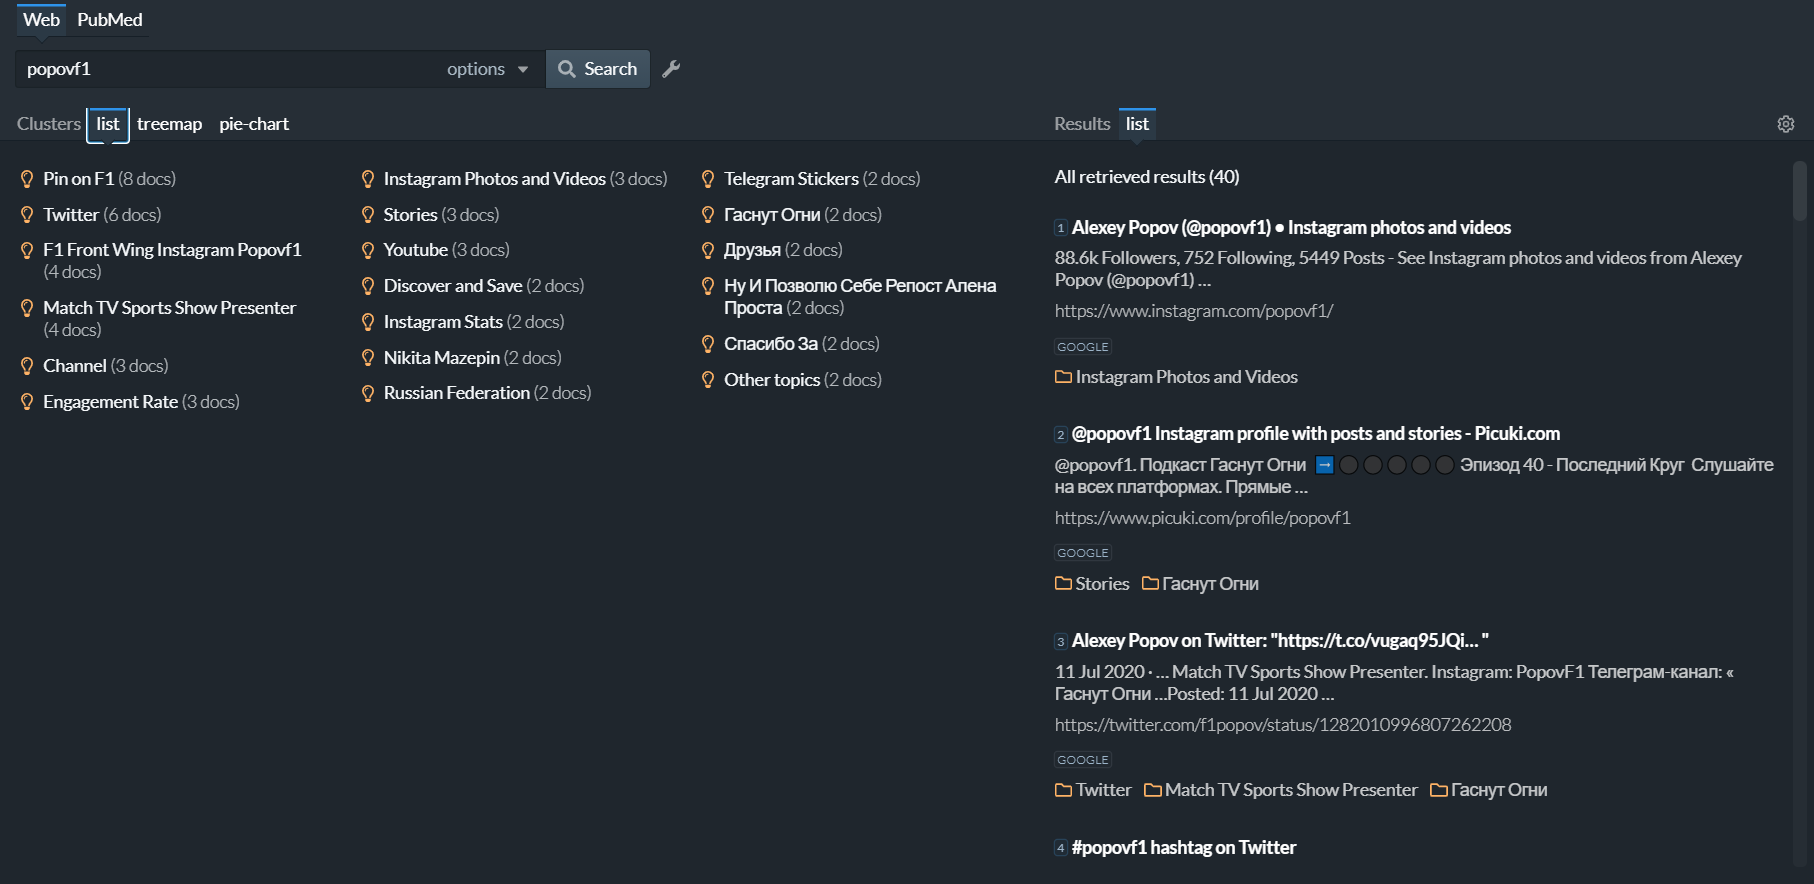
\includegraphics[height=6cm,keepaspectratio]{pictures/Carrot2_1.png}}
    \caption{Пример использования Carrot2 с разбиением результатов на группы.}
    \label{ris:image}
\end{figure}


\subsubsection{Yippy}
Yippy\footnote{http://yippy.com/} -- это метапоисковый движок, который группирует результаты поиска на категориям в группы.
Наделен обширным функционалом: позволяет искать по ключевым словам новости, вакансии, правительственную информацию и блоги.
Также позволяет вручную настраивать источники данных для собственного уникального метапоиска. \cite{yippywikipedia}

Преимущества:
\begin{itemize}
    \item группирует данные по тематическим категориям;
    \item есть возможность поиска не только ссылок в web-пространстве, но и непосредственно новостей, изображений и видео;
\end{itemize}

Недостатки:
\begin{itemize}
    \item сервис недоступен на территории РФ;
    \item нет поддержки GDQ.
\end{itemize}

\begin{figure}[H]
    \center{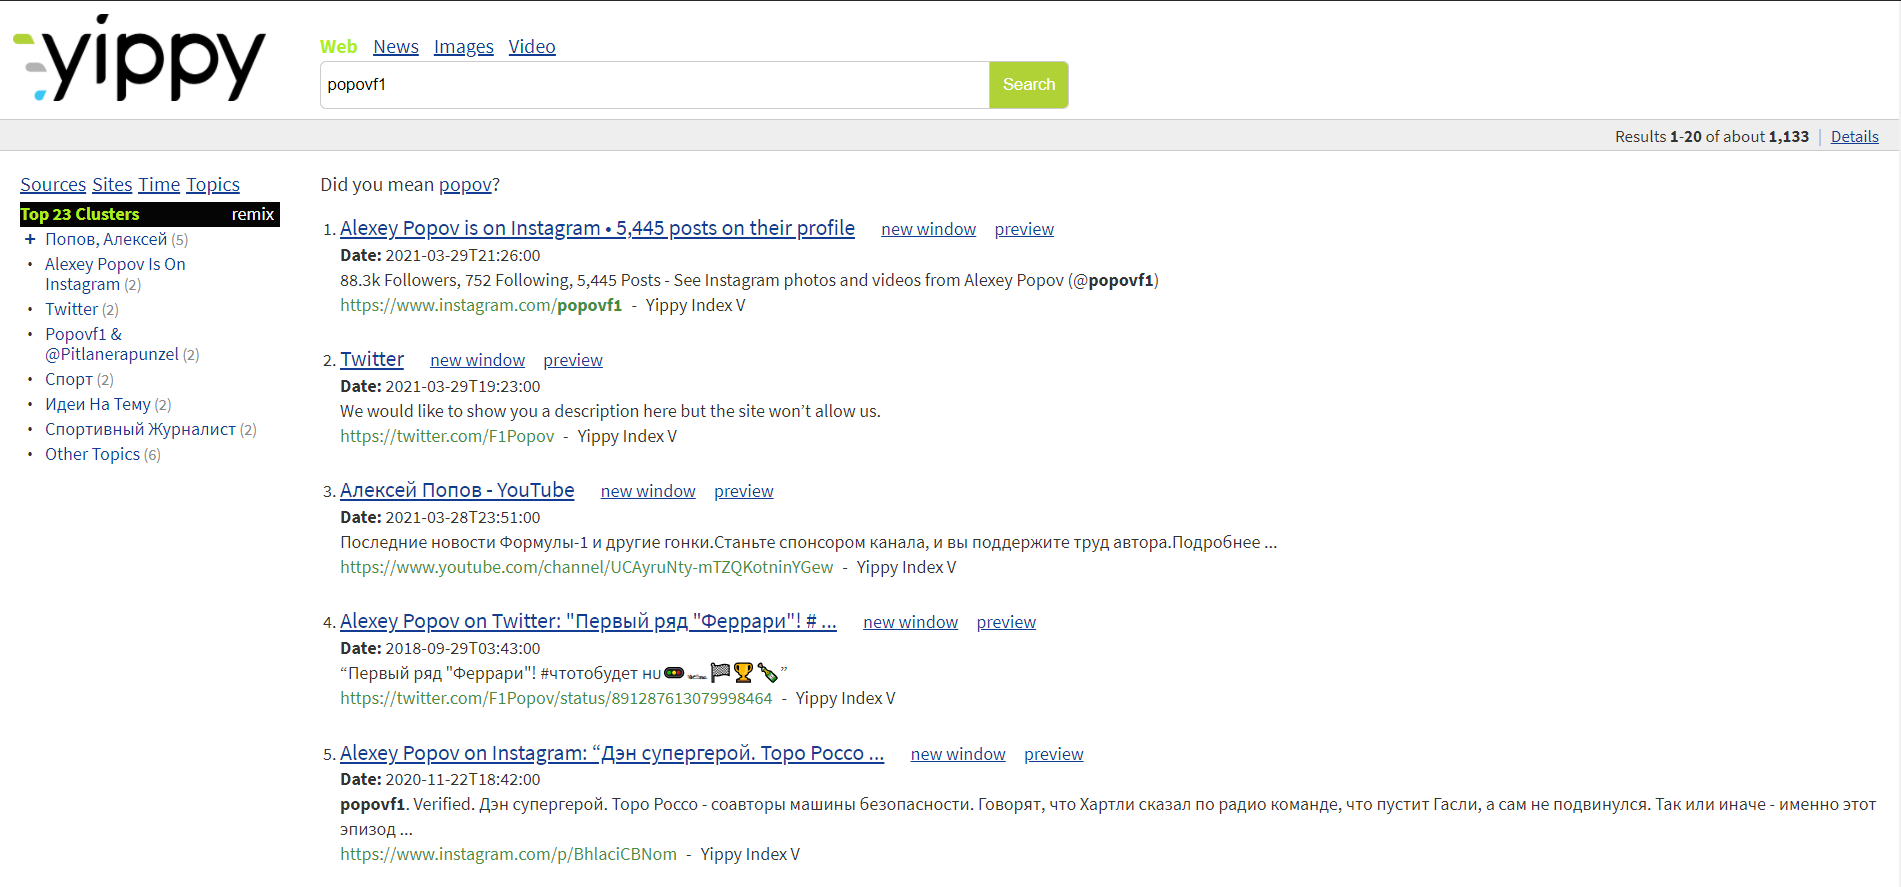
\includegraphics[height=6cm,keepaspectratio]{pictures/yippy_1.png}}
    \caption{Пример использования Yippy.}
    \label{ris:image}
\end{figure}

\subsection{Поиск данных в социальных сетях}
\subsubsection{Maltego}
Maltego\footnote{https://www.maltego.com/} -- это комплексное решение с множеством поддерживаемых источников информации.
Представляет из себя не движок, способный просто находить ссылки и группировать их, а проводит полноценный поиск и анализ
данных, выстраивает деревья взамосвязей. Например, может показать все активные адреса электронной почты заданного пользователя.
\cite{maltegohabr}

Преимущества:
\begin{itemize}
    \item выстраивание связей между объектами поиска, которыми могут быть как человек, так и группа лиц, компании, веб-сайты,
    организации и тому подобное;
    \item user-friendly интерфейс;
    \item возможность сохранения данных на стороне клиента с помощью СУБД;
    \item обладает гибкими настройками;
    \item является ПО с открытым исходным кодом, базовая версия которой поставляется абсолютно бесплатно в Kali Linux.
\end{itemize}

Недостатки:
\begin{itemize}
    \item для доступа ко всем возможностям программы необходимо оплачивать лицензию.
\end{itemize}


\subsubsection{ITools}
iTools\footnote{http://itools.com/search/people-search} -- это некий агрегатор всех инструментов, перечисленных выше. Имеет
возможности искать по ключевым словам людей и организаций во многих популярных современных социальных сетях. Для каждого из
подключенного метода поиска имеет свои настройки.

Преимущества:
\begin{itemize}
    \item большой перечень источников информации с настройками для каждого из них.
\end{itemize}

Недостатки:
\begin{itemize}
    \item нет никакой аналитики и сбора данных, просто поиск и ничего более;
    \item нет возможности запустить сбор по всем источникам одновременно;
    \item данные не собираются, не хранятся. Как следствие для полноценного использования необоходимо будет писать ПО поверх
    данного сервиса;
\end{itemize}

\begin{figure}[H]
    \center{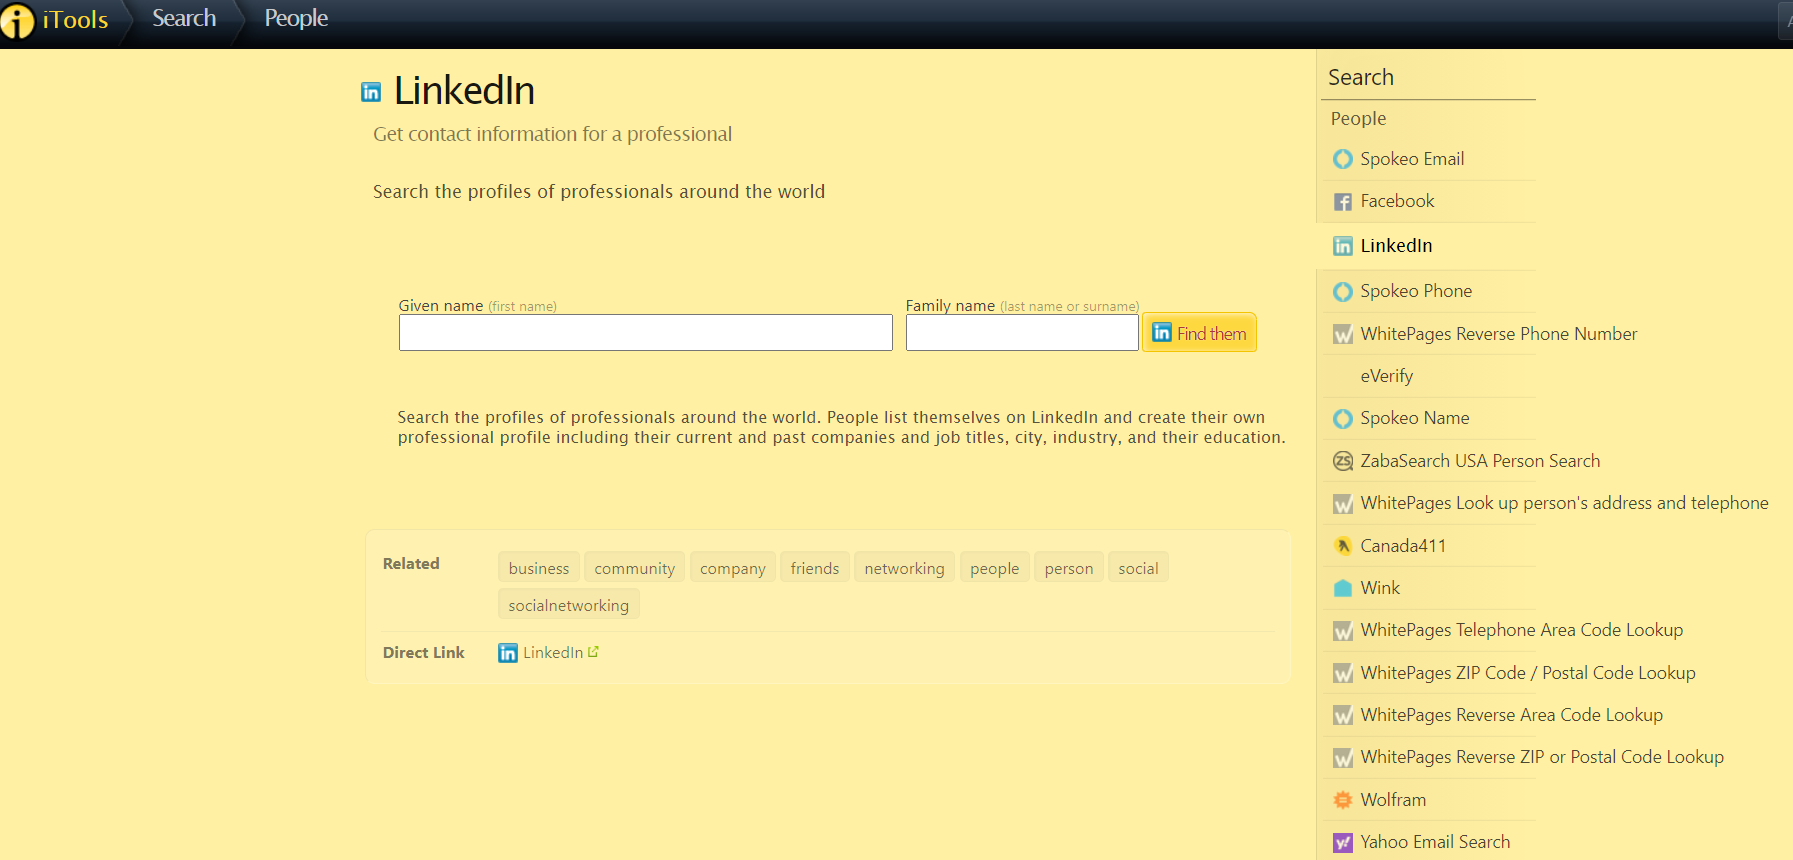
\includegraphics[height=6cm,keepaspectratio]{pictures/Itools_1.png}}
    \caption{Интерфейс агрегатора iTools.}
    \label{ris:image}
\end{figure}

\subsubsection{FindThatLead}
FindThatLead\footnote{https://findthatlead.com/en} -- это онлайн-сервис, позволяющий осуществлять поиск e-mail адресов
и страниц пользователей в социальных сетях LinkedIn и Twitter. Обладает возможностью проверять валидость найденного адреса
электронной почты. Главным отличием является то, что можно установить данное ПО как расширение браузера Chrome.

Преимущества:
\begin{itemize}
    \item лаконичный и понятный интерфейс, наличие расширения для браузера;
    \item поиск e-mail адресов по профилю в социальных сетях.
\end{itemize}

Недостатки:
\begin{itemize}
    \item анализ данных можно совершить только вручную;
    \item малое количество собираемой информации;
    \item не подходит для комплексного и обширного анализа сущностей.
\end{itemize}

\begin{figure}[H]
    \center{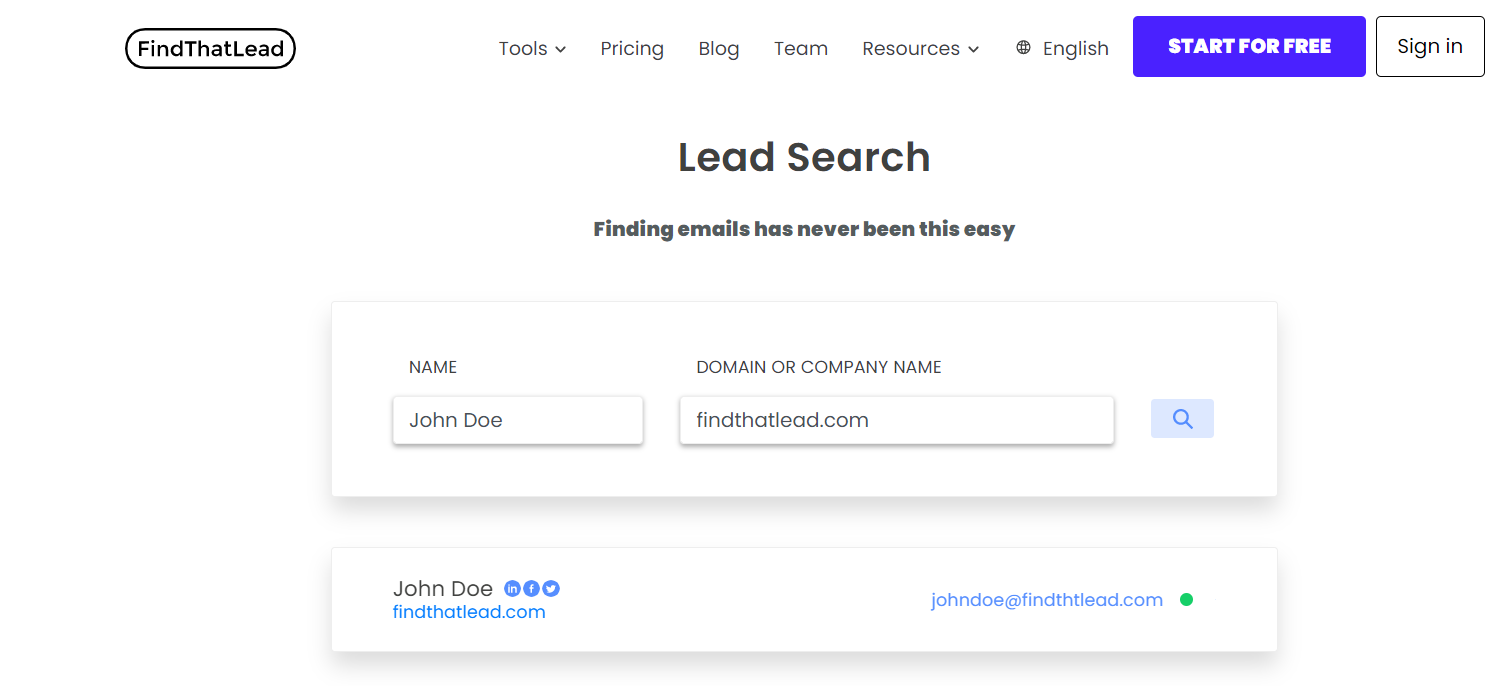
\includegraphics[height=6cm,keepaspectratio]{pictures/findthatlead_1.png}}
    \caption{Интерфейс FindThatLead.}
    \label{ris:image}
\end{figure}

\subsection{Универсальные приложения}
\subsubsection{Виток OSINT}
Виток OSINT\footnote{https://norsi-trans.ru/catalog/vitok-osint/} -- это отечественное решение для спецслужб, позволяет собирать
информацию с помощью поисковых сервисов, так и анализируя данные социальных сетей. Строит деревья зависимостей между объектами
поиска, которыми могут быть: человек, организация, событие. Имеет индексацию и дедупликацию данных, в следствие чего система
не перегружена излишками данных и повышает проиводительность. Вся информация также имеет привязку к географическому положению, что
позволяет более наглядно воспринимать собранные и проанализированные ПО данные.

\par
Главным и единственным недостатком является приватность системы, программы нет в свободном доступе и оценить ее возможности
вживую не представляется возможным.

\subsubsection{Palantir}
Palantir\footnote{https://www.palantir.com/solutions/intelligence/} -- это зарубежное решение для спецслужб, делающее ставку 
прежде всего на безопасность собранной информации, удобную и развернутую подачу последней. Присутствует возможность как просто
получать информацию из социальных сетей и прочих открытых источников, так и наблюдать за видеопотоком с камер наблюдений. Имеет
визуализацию на карте мира.


\par
Главным и единственным недостатком является приватность системы, программы нет в свободном доступе и оценить ее возможности
вживую не представляется возможным.

\subsection{Выводы}
В результате исследования существующих методов сбора информации были выделены два подхода: поиск с помощью поисковых сервисов;
поиск внутри социальных сетей. Однако большинство решений, которые произвоидили поиск через поисковые сервисы, зачастую не могли
предоставить полноценный сбор и анализ данных, которые можно было б в последствии загрузить в СУБД для отображения в каком-либо
интерфейсе. Пожалуй, это главный недостаток приложений с таким подходом. Второй путь, поиск внутри соц сетей -- зачастую реализован
только в коммерческих проектах, и проверить объем извлекаемых данных невозможно.